\section{La Norma ISDB-T}
%\subsection{Conceptos generales sobre la norma}*
\begin{frame}{La Norma ISDB-T}
	\begin{block}{Las Normas o Estándares}
	\begin{itemize}
		%\subsection{Las Normas o Estandares}
		\item {	¿Qué es una norma?}
		\item { ¿Qué alcance tiene la norma? }
		\item {	¿Cómo se define una norma?	}
	\end{itemize}
	\end{block}
	\begin{block}{La Norma ISDB-T}
	\begin{itemize}
		%\subsection{Las normas de Television Digital}
		\item {	Normas existentes en la actualidad}
		\item { Los países y las normas que usan }
		\item {	Uruguay y la definición por ISDB-T	}
	\end{itemize}
	\end{block}
\end{frame}

\begin{frame}{La Norma ISDB-T}
%\begin{block}{Conceptos básicos}
\begin{figure}
	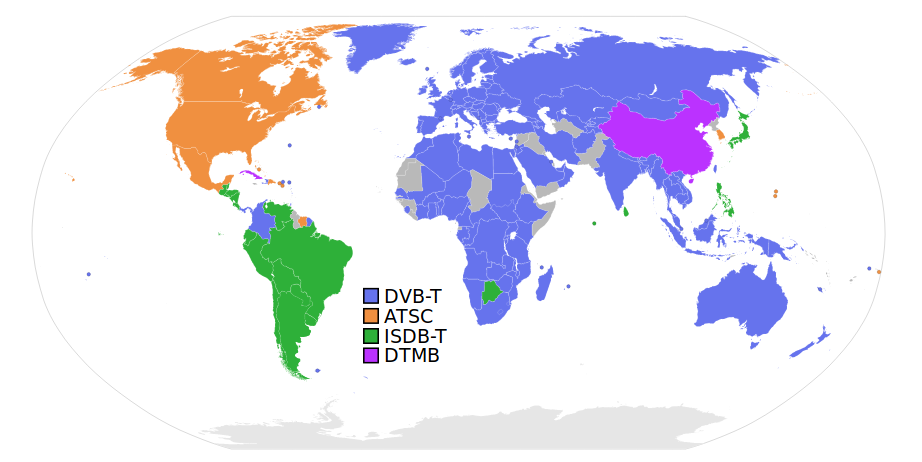
\includegraphics[scale=0.35]{Standards}
	%\caption{Distribución de las normas de TVD en el mundo}
\end{figure}
%\end{block}

\end{frame}

%\subsection{ISDB-T, la norma japonesa-brasilera de televisión}*
\begin{frame}{La Norma ISDB-T}
	\begin{block}{ISDB-T}
	\begin{itemize}	
		\item {	La entrada de datos}
		\item { Las capas jerárquicas}
		\item {	Robustecimiento a nivel datos y a nivel portadora}
		\item { OFDM }
	\end{itemize}
\end{block}
\end{frame}

%		\begin{frame}{Blocks}
%			\begin{block}{Block Title}
%			You can also highlight sections of your presentation in a block, with it's own title
%			\end{block}
%			\begin{theorem}
%			There are separate environments for theorems, examples, definitions and proofs.
%			\end{theorem}
%			\begin{example}
%			Here is an example of an example block.
%			\end{example}
%		\end{frame}
